%!TEX ROOT=../dissertation.tex
% UZAVŘENO! ÚPRAVY JEN ŽIVOTNĚ NUTNÉ NEBO VE ZBYLÉM ČASE


\chapter{FEVER CS: a Dataset Localization}
\label{chap:fever_cs}
In Chapter~\ref{chap:collection}, we have examined the existing datasets for our task. In this chapter, we will attempt to extract a part of the correct fact verification examples they carry, and localize them into Czech. More specifically, we will be proposing localization methods for the greatest one -- the \textsf{FEVER} dataset.

Even though the localization process is prone to imperfections of all sorts, its resulting dataset will be of great use training the \textit{baseline} models, as well as \textit{pre-training} the finer models in the later stages of our work, when a native Czech dataset will be introduced for the \textit{fine-tuning}.
\section{FEVER format}
Before we start to extract the Czech $(claim,evidence)$ pairs, let us examine the format of the \textsf{FEVER} datapoints.

\begin{figure}[H]
\begin{lstlisting}[language=json]
{
  "id": 36242,
  "verifiable": "VERIFIABLE",
  "label": "REFUTES",
  "claim": "Mud was made before Matthew McConaughey was born.",
  "evidence": [
    [
      [52443, 62408, "Mud_-LRB-2012_film-RRB-", 1],
      [52443, 62408, "Matthew_McConaughey", 0]
    ],
    [
      [52443, 62409, "Mud_-LRB-2012_film-RRB-", 0]
    ]
  ]
}
\end{lstlisting}
    \caption{Example \textsf{FEVER} \texttt{REFUTES} annotation with two possible evidence sets}
    \label{list:fever}
\end{figure}

\begin{itemize}
    \item Dataset is stored in \texttt{JSON} Lines (\texttt{JSONL}) format, each line features a data point like~\ref{list:fever} without the whitespace
    \item The verifiability is stored in attribute $\texttt{verifiable}\in\{\texttt{VERIFIABLE},\texttt{NOT VERIFIABLE}\}$, veracity is stored using $\texttt{label}\in\{\texttt{SUPPORTS},\texttt{REFUTES},\texttt{NOT ENOUGH INFO}\}$ 
    \item \texttt{evidence} is a set of all possible \textit{evidence sets}, any of these sets \textit{alone} suffices to refute the \texttt{claim}
    \item Every such an \textit{evidence set} is structured as a conjunction of \textsf{Wikipedia} sentences in format: \texttt{[annotation\_id, evidence\_id, article\_wikiid, sentence\_index]}
    
\end{itemize}

\noindent To illustrate the correct interpretation of data from the example~\ref{list:fever}, there are two possible counterproofs for the claim \"{\textit{Mud was made before Matthew McConaughey was born.}}:

\begin{figure}[H]
    \centering

    \textit{Evidence set \#1:}
    \begin{ctucolortab}
    
    \fbox{\begin{minipage}{0.9\textwidth}
       \begin{hangparas}{2em}{1}
            \textbf{[Mud (film)]} Mud is a 2012 American coming-of-age drama film written and directed by Jeff Nichols.
            
            \textbf{[Matthew McConaughey]} Matthew David McConaughey (born November 4, 1969) is an American actor.
            
        \end{hangparas}
    \end{minipage}}
    \end{ctucolortab}

    ~
    
    \textit{Evidence set \#2:}
    
    \begin{ctucolortab}
    \fbox{\begin{minipage}{0.9\textwidth}
       \begin{hangparas}{2em}{1}
            \textbf{[Mud (film)]} The film stars Matthew McConaughey, Tye Sheridan, Jacob Lofland, Sam Shepard, and Reese Witherspoon.
        \end{hangparas}
    \end{minipage}}
    \end{ctucolortab}
    \caption{Evidence from data point~\ref{list:fever}}    
    \label{fig:evidence}
\end{figure}

\section{Localizing the FEVER}
\label{sec:fevercs}
Before we introduce the single steps, let us design a simple scheme for localizing it into an arbitrary language exploiting the ties between \textsf{FEVER} and \textsf{Wikipedia}:

Starting from the \textsf{FEVER}~\cite{fever} dataset:
\begin{enumerate}
    \item Merge the \textsf{FEVER} \textsf{train} and \textsf{dev} datasets into a joint dataset \textsf{fever\_en}
    \item Using \textsf{MediaWiki API}, map every \textsf{Wikipedia} article used in \textsf{fever\_en} evidences to its target localization, if none found, remove every \textit{evidence set} that contains it to create the \textsf{fever\_lang} -- in our case, the \textsf{fever\_cs} (Section~\ref{sec:fever-loss})
    \item Remove all \texttt{SUPPORTS} and \texttt{REFUTES} data points with empty evidence from \textsf{fever\_lang} 
        \item Download the current \textsf{Wikipedia} dump in the target language, parse it into a \textit{knowledge base} -- plain text corpus keyed by article name (Section~\ref{sec:wikidump})
    \item Localize every claim using the Machine Translation (Section \ref{sub:mach})
    \item Normalize every string value in \textsf{fever\_lang}, as well as the knowledge base, using the same Unicode normal form (Section~\ref{sub:canonical})
    \item Sample around $0.05\cdot|\textsf{fever\_lang}|$\footnote{This split size is proportional to that of \textsf{FEVER EN} -- it balances the labels to punish bias and favours the \textsf{train} size, due to the data-heavy nature of the task} annotations for each label using a fixed \textit{random seed}\footnote{This ensures the reproducibility}, store them as \textsf{dev}. Repeat for \textsf{test}.
    \item Store the rest of labels as \textsf{train}
\end{enumerate}

This scheme has notable weaknesses. Firstly, the evidence sets are not guaranteed to be exhaustive -- no human annotations in the target language were made to detect whether there are new ways of verifying the claims using the target version of \textsf{Wikipedia}. Furthermore, an unknown number of evidence has lost its validity, as the given \textsf{Wikipedia} localization lacks the specific information needed to conclude the fact-checking verdict.

With all of the dataset's flaws listed above to keep in mind, it is an exciting starting point, appropriate for training and validating both the early Document Retrieval and Natural Language Inference models. Therefore, we argue, it is a fruitful experimental dataset for both fields of our research.

Now, let us reinforce on the non-trivial points from the scheme above, specifically for our Czech instance.
\subsection{Czech Wikipedia (June 2020) corpus}
\label{sec:wikidump}
As an experimental \textit{knowledge base}, we are providing the \textsf{CS June 2020 Wikipedia dump} parsed into a plain text corpus using the \textsf{WikiExtractor} and structured into a \textsf{FEVER-}like knowledge base, i.e., a \textsf{SQLite} single-table\footnote{The table name is \db{Document}} database, providing every article \textit{abstract} from the \textsf{CSWiki} dump, structured as its \texttt{id}, \texttt{text} and its \texttt{sentences}-split, computed using the \textsf{Punkt}~\cite{punkt} sentence tokenizer. 

The resulting knowledge base can be downloaded from our webpage\footnote{\url{http://bertik.net/cswiki}} and the tools for its extraction are open-sourced in the section~\ref{sec:fever_result}.

\subsection{Localization data loss}
\label{sec:fever-loss}
For every article, \textsf{Wikipedia} provides a set of links to the same article in different foreign languages. This feature is powered by the \textsf{MediaWiki} database and can be accessed programatically through the \textsf{MediaWiki API}~\cite{mediawiki}. 

In the early stage of development, we have written the ad--hoc \textsf{localize\_dataset}\footnote{\url{https://github.com/heruberuto/fact-checking/blob/master/localize_dataset.py}} \textsf{Python} module to exploit this feature. Its outputs for the \texttt{cs} target language (measuring the \textit{data loss} in the step 2. of~\ref{sec:fevercs}) are \textit{highly} encouraging:

\begin{lstlisting}
    Of 12633 articles: 6578 preserved, 6055 lost, of which 84 due to normalization
    Of 145449 data points, 112969 survived the localization (of which 35639 was not verifiable), 32480 didn't
\end{lstlisting}

That means the majority of \textsf{FEVER-}adjacent articles \textit{do} have their Czech translation, and, even more surprisingly, whole \textbf{78\%} of claims can be fully (dis-)proven in at least one way using only the Czech \textsf{Wiki}. That is, in an ideal world where the Czech abstracts are semantically equivalent to their English counterparts and no \texttt{NOT ENOUGH INFO} annotations are lost due to a piece of knowledge unique to \textsf{CSWiki}.

Still, this is most often the case for the points we examined, and even though the original sentence indices from~\ref{list:fever} can not be trusted, the \texttt{wikiid} typically can. The \textit{precision/recall} (\ref{sec:recall}) metrics are yet to be done using human annotations, however, the empirical intuition would be that \textit{recall} took most of the damage (\textit{evidence sets} \"{forgotten} by our dataset).
\subsection{Tested Approaches for English-Czech Machine Translation}
\label{sub:mach}
As the Machine Translation model evaluation is a complex field of its own, and as the standard metrics such as BLEU~\cite{bleu} or SacreBLEU~\cite{sacrebleu} require a number of human-annotated reference translations, we do not possess the time to properly cover it in our research project. Thus, we are down to our own empirical observations of the translation quality. Our conclusions should be taken as such.

From the tools openly available online in a ready-to-use manner, we have examined the following (Table~\ref{fig:translators}):

\begin{enumerate}
    \item {\techbf{Google Cloud Translation API}}~\cite{google} was the platform we used to translate the first version of FEVER CS dataset, as it is convenient to use on a large set of data, and as it empirically yielded a \textit{comprehensible} translation for the majority of~claims.
    \item {\techbf{LINDAT Translation Service}}~\cite{lindat} uses {\textsf{CUBBITT}}~\cite{Popel2020} transformer model for machine translation and was released after its publication in \textsf{Nature} in September 2020. It performs on par with the top commercial-grade translators, however, it is published under a restrictive license for personal use.
    \item {\techbf{DeepL}}~\cite{deepl} released its English--Czech translation model for public use on March $17^{th}$ 2021. While we found out about it two weeks before the thesis submission deadline, we feature its outputs in the final dataset, as we have observed its translations to be superior both in the \textit{translation adequacy}\footnote{Preserving text meaning~\cite{Popel2020}} and the fluency of the resulting texts. We have found it to be very robust against homonyms\footnote{Words that can have different meanings (and therefore different Czech translations), which, typically, must be guessed from the context -- s. a. the \"{river \textit{bank}} and the \"{retail \textit{bank}}}, which is crucial for preserving the claim meaning and, therefore, the validity of transferred evidence.
\end{enumerate}

%---- TEXTBOX=TRANSLATORS
\begin{table}[H]
\begin{ctucolortab}
\begin{tabular}{ l r r | l }

    
    \textbf{Original claim} &\footnotesize{EN}& ~ & \textbf{\"{Harald V of Norway married a commoner.}}\\
    \hline
    \textbf{\textsf{Google Translate}} &\footnotesize{CS}&\footnotesize{April'20}& \"{Norská Harald V se oženila s občanem.}\\
    \textbf{\textsf{Google Translate}} &\footnotesize{CS}&\footnotesize{May'21}& \"{Harald V Norska si vzal prostého občana.}\\
    \textbf{\textsf{CUBBITT}} &\footnotesize{CS}&\footnotesize{May'21} & \"{Harald V. z Norska si vzal neurozenou ženu.}\\
    \textbf{\textsf{DeepL}} &\footnotesize{CS}&\footnotesize{May'21} & \"{Harald V. Norský se oženil s obyčejnou ženou.}\\
    \hhline{===|=}
    \textbf{Original claim} &\footnotesize{EN}& ~ & \textbf{\"{Indiana Jones has been portrayed by an actor.}}\\
    \hline
    \textbf{\textsf{Google Translate}} &\footnotesize{CS}&\footnotesize{April'20}& \"{Indiana Jones byl vylíčen hercem.}\\
    \textbf{\textsf{Google Translate}} &\footnotesize{CS}&\footnotesize{May'21}& \"{Indiana Jones byl zobrazen hercem.}\\
    \textbf{\textsf{CUBBITT}} &\footnotesize{CS}&\footnotesize{May'21} & \"{Indiana Jonese ztvárnil herec.}\\
    \textbf{\textsf{DeepL}} &\footnotesize{CS}&\footnotesize{May'21} & \"{Indiana Jones byl ztvárněn hercem.}\\
    \hhline{===|=}
    \textbf{Original claim} &\footnotesize{EN}& ~ & \textbf{\"{Manchester by the Sea has grossed money.}}\\
    \hline
    \textbf{\textsf{Google Translate}} &\footnotesize{CS}&\footnotesize{April'20}& \"{Manchester u moře rozdal peníze.}\\
    \textbf{\textsf{Google Translate}} &\footnotesize{CS}&\footnotesize{May'21}& \"{Manchester by the Sea vydělal peníze.}\\
    \textbf{\textsf{CUBBITT}} &\footnotesize{CS}&\footnotesize{May'21} & \"{Manchester by the Sea utržil peníze.
}\\
    \textbf{\textsf{DeepL}} &\footnotesize{CS}&\footnotesize{May'21} & \"{Film Manchester by the Sea vydělal peníze.}\\
\end{tabular}
\end{ctucolortab}
\caption[Machine Translator comparison using \textsf{FEVER} claims]{Machine Translator comparison using \textsf{FEVER} claims. Examples were cherry-picked to highlight the observed differences between translators.}
    \label{fig:translators}
\end{table}

%---- /TEXTBOX

\subsection{Unicode Normalization}
\label{sub:canonical}
 In the Unicode paradigm, the same diacritized character can be stored using several different representations~\cite{unicode}. To allow straightforward byte-wise comparisons on the low level (s. a. TF-IDF search, neural networks, \dots), one should eliminate this property using one of the \textit{Unicode normal forms}:
 
\begin{enumerate}
    \item {\techbf{NFD}} -- \textit{Normalization Form Canonical Decomposition} -- fully expands out the character (see Figure~\ref{fig:unicode}). Is faster to compute, but ultimately takes more space. Theoretically, it could be used to exploit the property of Czech, that the words that have similar undiacritized representations tend to be semantically close (e. g. \"{býti} and \"{bytí} share 4 bytes rather than 2 in NFD)
    \item {\techbf{NFC}} -- \textit{Normalization Form Canonical Composition} -- runs the NFD algorithm and then combines the characters where possible -- it runs longer, but the resulting strings take up less space
\end{enumerate}

%--- FIG: UTF forms
\begin{figure}[H]
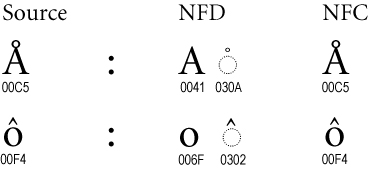
\includegraphics[width=6cm]{fig/UAX15-NormFig4.jpg}
\caption{Unicode normal forms, reprinted from~\cite{unicode}}
\label{fig:unicode}
\end{figure}
%--- /FIG

\subsection{Document leakage}
\label{sec:leakage}
An interesting and possibly malicious property of our dataset is a large \textit{document leakage} due to the simplistic splitting strategy defined in \ref{sec:fevercs} step 9.

Simply put, the \textsf{train} and \textsf{test} splits may contain claims related to the same evidence-set document. However, this was neither addressed by~\cite{fever}, as we have found \textbf{11,165} out of their \textbf{13,332} \textsf{dev}\footnote{Only the \texttt{SUPPORTS} and \texttt{REFUTES} annotations are considered in our measure, as the \texttt{NEI}s do not carry any evidence to compare against.}  annotations sharing an evidence-set document with some \textsf{train} claim. 

A further research is needed to answer whether this is a problem and what are the optimal strategies to punish model \textit{overfitting} while still optimizing for a broad topic coverage, proportional to the number of  leakage-prone documents.

\section{Resulting Dataset}

\label{sec:fever_result}
\begin{table}[H]
\begin{ctucolortab}
\begin{tabular}{ l | l l l || l l l  }
&  {\techbf{{FEVER CS}}} & & & {\techbf{{FEVER EN}}}&&\\
{} & {\texttt{SUPPORTS}} & \texttt{REFUTES}  & \texttt{NEI} & {\texttt{SUPPORTS}} & \texttt{REFUTES}  & \texttt{NEI}\\ 
\hline
{\tech train} & 53,542 & 18,149 & 35,639 & 80,035 &29,775& 35,639
\\
{\tech dev} & 3,333 & 3,333 & 3,333 & 6,666 & 6,666 & 6,666\\
{\tech test} & 3,333 & 3,333 & 3,333& 6,666 & 6,666 & 6,666\\
\end{tabular}
\end{ctucolortab}
\caption{Label distribution in \textsf{FEVER CS} dataset as oposed to the \textsf{FEVER EN}}
\label{tab:fevercs-overview}
\end{table}


In Table~\ref{tab:fevercs-overview} we show the label distribution in our dataset, is roughly proportional to that in \textsf{FEVER EN}. Inspired by the~\cite{fever} paper that only uses a \textsf{dev}, \textsf{test} of 3,333 claims per annotation to establish the baseline models, we have opted the same split size. This decision was experimental and should be further challenged in the future. 

Following the scheme described in~\ref{sec:fevercs}, we have released its open source implementations\footnote{\url{https://github.com/aic-factcheck/fever-cs-dataset}}~\footnote{\url{https://github.com/heruberuto/fact-checking/}} for an arbitrary language, and a set of ready-made \textsf{train}, \textsf{test} and \textsf{dev} data\footnote{\url{http://bertik.net/fever-cs}} in its most recent version Machine-Translated by \textsf{DeepL}. Both the data and the implementations are being published under the \textsf{CC BY-SA 3.0} license.
